\documentclass[class=book, crop=false, oneside]{standalone}
\usepackage[subpreambles=true]{standalone}

\usepackage{../../style}

\graphicspath{{./assets/images/}}

% arara: pdflatex: { synctex: yes, shell: yes }
% arara: latexmk: { clean: partial }
\begin{document}
\chapter{La gerarchia di memoria}

\section{Introduzione}
Sottolineare quanto il concetto di memoria sia importante e necessario nei dispositivi elettronici del giorno d'oggi risulta abbastanza scontato. D'altra parte, viene fatta subito una precisazione: non esiste un'unica soluzione che permette di ottenere la memoria "perfetta". Esistono infatti diverse implementazioni, ognuna con i suoi compromessi, che variano per costo, prestazioni e capacità.

\section*{Qualche definizione}
Possiamo distinguere principalmente due tipologie di memoria in base alla modalità di accesso:
\begin{itemize}
	\item \emph{memoria indirizzata direttamente} (memoria principale, memoria cache):
	\begin{itemize}
		\item è volatile, ossia il suo contenuto viene perso se viene spento il calcolatore;
		\item è limitata per capacità dallo spazio di indirizzamento definito dall'architettura del processore;
		\item i dati contenuti nella memoria principale sono disponibili in qualsiasi momento;
	\end{itemize}
	\item \emph{memoria indirizzata indirettamente} (memoria periferica):
	\begin{itemize}
		\item è di tipo permanente, ossia mantiene il suo contenuto anche senza alimentazione;
		\item ha uno spazio di indirizzamento software che non dipende dall'architettura del processore;
		\item i dati contenuti nella memoria periferica devono essere trasferiti alla memoria principale prima di essere utilizzati (solitamente questo processo viene mediato dal software, tipicamente il sistema operativo);
	\end{itemize}
\end{itemize}

A seguire un elenco di definizioni che utilizzeremo in seguito:
\begin{itemize}
	\item \emph{Tempo di accesso}: è il tempo richiesto per \emph{una} operazione di lettura / scrittura nella memoria;
	\item \emph{Tempo di ciclo}: è il tempo che intercorre fra l'inizio di due istruzioni consecutive; è composto dal tempo di accesso sommato al tempo per muovere il dato con cui si stava lavorando;
	\item \emph{Accesso casuale}: è quella modalità di accesso in cui non vi è alcun ordine o relazione fra i dati memorizzati; è tipico delle memorie a semiconduttori;
	\item \emph{Accesso sequenziale}: è quella modalità che presuppone lo scorrimento ordinato di un blocco di dati per accere ad un suo dato; il tempo d'accesso dipende dalla posizione fisica del dato nel supporto (tipicamente nastri e dischi);
	\item \emph{RAM} (\emph{Random Access Memory}): è una memoria dotata di accesso casuale che permette scrittura e lettura; viene implementata attraverso semiconduttori;
	\item \emph{ROM} (\emph{Read Only Memory}): è una memoria a semiconduttori che prevede solo un accesso in lettura; esistono implementazioni sia attraverso accesso casuale che sequenziale
\end{itemize}

\section{La memoria principale}
\subsection{Le RAM}
Descriviamo come avviene la connessione logica fra memoria RAM e CPU:
\begin{figure}[H]
	\centering
	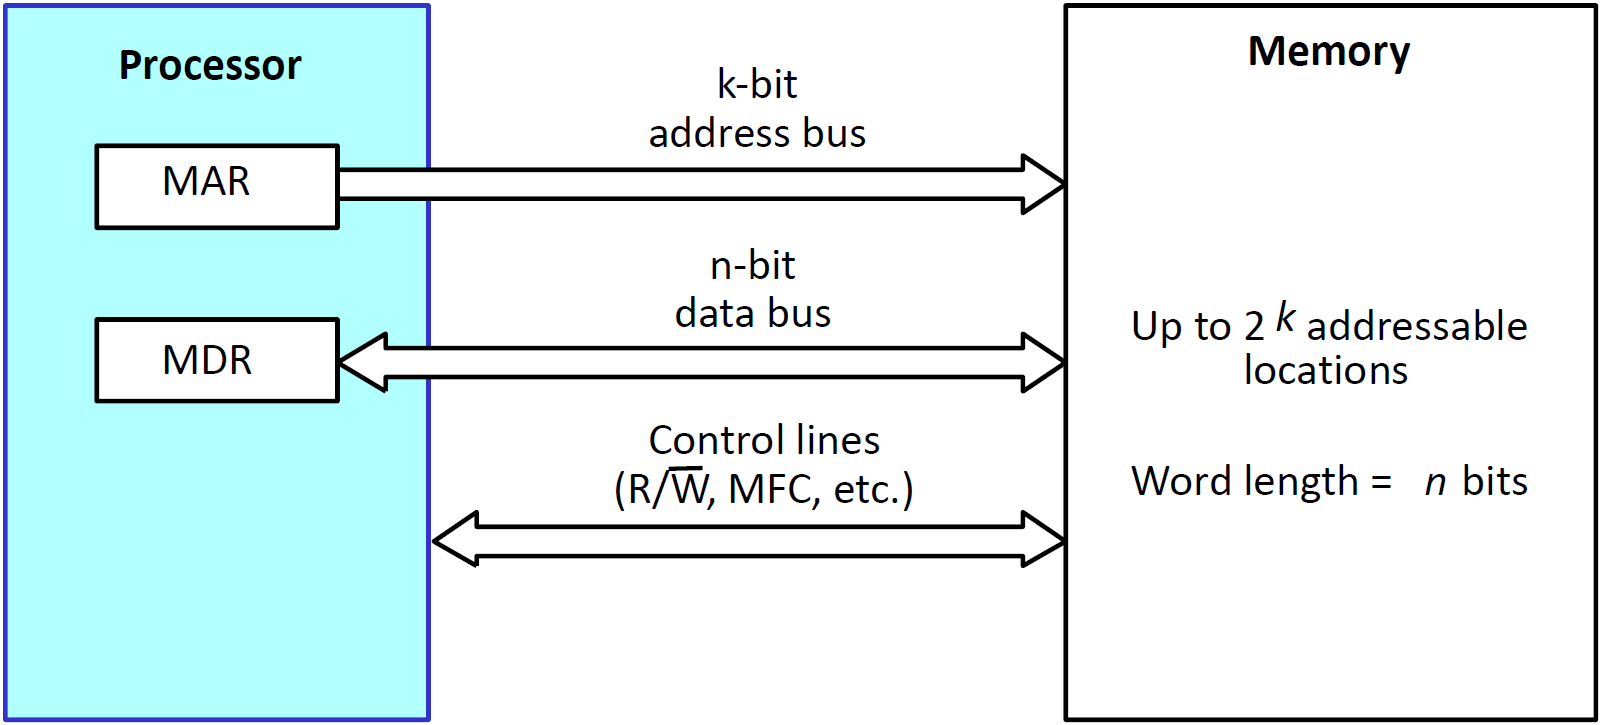
\includegraphics[width=\textwidth,keepaspectratio]{relazione_cpu_ram.png}
	\caption{Modello della relazioni logiche fra CPU e RAM}
\end{figure}

\subsection{Le SRAM}

\subsection{Le DRAM}







\end{document}
